\newpage
\section{Vorbereitung}
In der Vorlesung wird als Beispiel eines RTOS das FreeRTOS behandelt. Lesen Sie in der Dokumentation zu FreeRTOS (\url{http://www.freertos.org}) im Quick Start Guide und der API, wie in FreeRTOS Tasks angelegt und benutzt werden. Datenblatt des Fototransistors: \url{http://www.mouser.com/ds/2/311/SFH\%20309,\%20SFH\%20309\%20FA,\%20Lead\%20(Pb)\%20Free\%20Product\%20-\%20RoHS-368614.pdf}
\begin{figure}[h!]
	\centering
	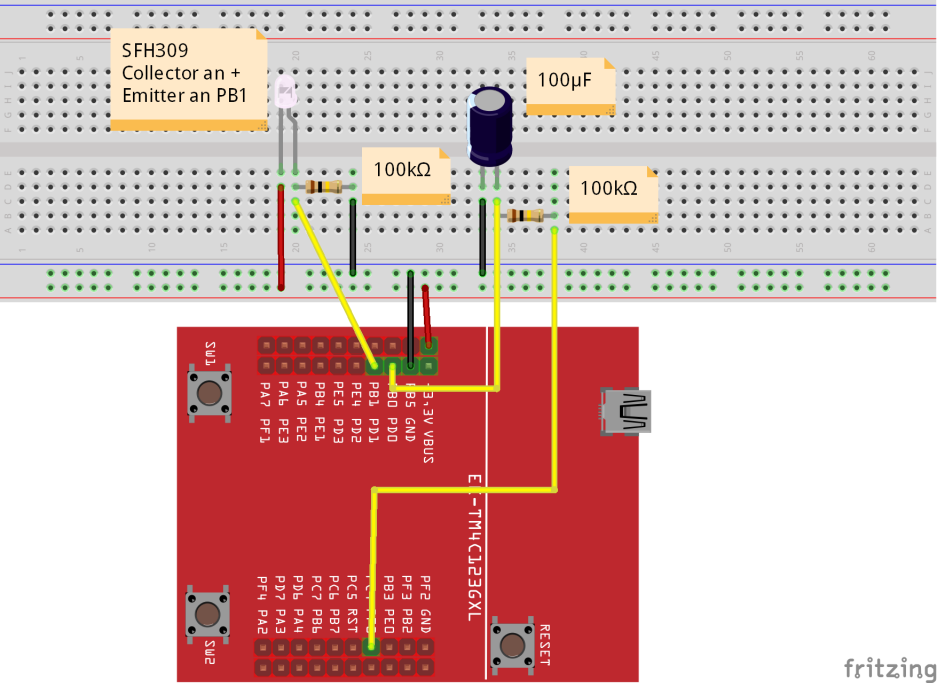
\includegraphics[width=0.7\linewidth]{images/Schaltplan6}
\end{figure}

\noindent Das Schaltbild zeigt eine RC-Kombination (Widerstand und Elektrolytkondensator) und einen Fototransistor zur Simulation eines Systems mit Temperaturregelung. Die Kapazität des Kondensators stellt dabei die Temperatur und der Widerstand die Heizung sowie Kühlung dar.\\ \\
Es sollen nun zwei Prozesse/Tasks laufen. Ist der erste Task aktiv, wird er jede Sekunde aufgerufen. Der zweite Task hat eine höhere Priorität als der erste und wird alle zwei Sekunden aufgerufen.\\ \\
In dem ersten Task wird die aktuelle Temperatur (=Spannung des Kondensators) ermittelt. Es wird unterschieden in Heizen und Kühlen. Beim Heizen (= Aufladen des Kondensators) wird solange Energie zugeführt, bis der ausgelesene Wert z.B. 600 Einheiten überschreitet. Dann findet das Kühlen (=Entladen) solange statt, bis der Wert z.B. 300 Einheiten unterschreitet. Nach einem Unterschreiten wird wieder das Heizen durchgeführt usw.\\ \\
Der zweite Task überwacht die Helligkeit und regelt, dass die Heizung nur bei einer Helligkeit kleiner als z.B. 200 Einheiten aktiv ist.
\section{Aufgabe 1}
Modellieren Sie das beschriebene System mit einen Statechart. Skizzieren Sie die Aktivität der Prozesse exemplarisch als Zeitverlaufsdiagramm.\\ \\
\begin{figure}[h!]
	\centering
	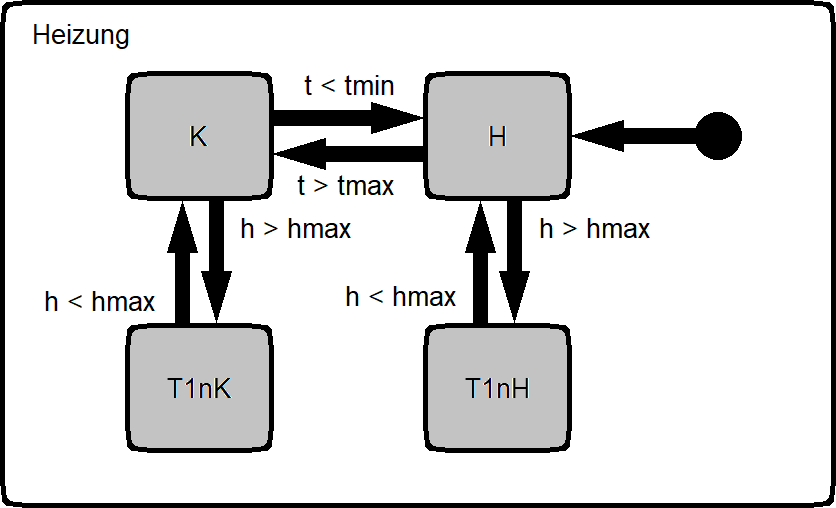
\includegraphics[width=0.7\linewidth]{images/Statechart}
\end{figure}
\begin{itemize}
	\item K = kühlen
	\item H = heizen
	\item T1nK = Task 1 nickt aktiv, letzter Zustand kühlen
	\item T1nH = Task 1 nickt aktiv, letzter Zustand heizen
	\item h = Helligkeit
	\item hmax = max Helligkeit
	\item t = Temperatur
	\item tmax = min Temperatur
	\item tmin = min Temperatur
\end{itemize}
\begin{figure}[h!]
	\centering
	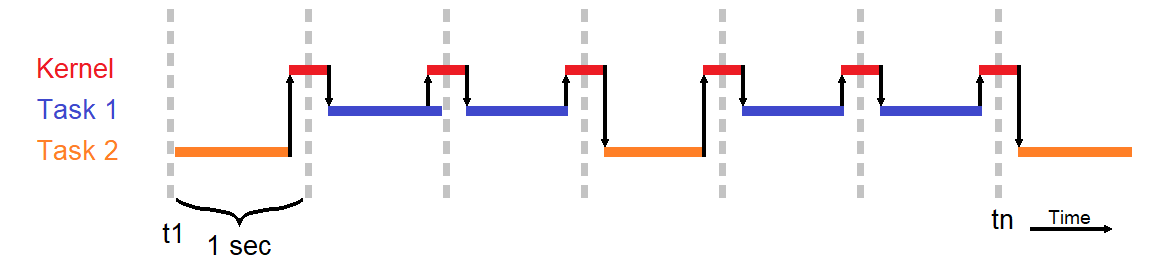
\includegraphics[width=0.7\linewidth]{images/Zeitverlaufsdiagramm}
\end{figure}

\section{Aufgabe 2}
Bauen Sie die dargestellte Schaltung auf und fügen Sie dieser eine LED (mit Vorwiderstand, 150 $\Omega$) hinzu, so dass die LED leuchtet, wenn gerade geheizt wird. Die LED ist in die Schaltung zu integrieren, ohne dass ein weiterer Port des LaunchPads verwendet wird. D.h. das Programm für das LaunchPad in der nächsten Aufgabe soll die LED nicht explizit betrachten.\\ \\
\begin{figure}[h!]
	\centering
	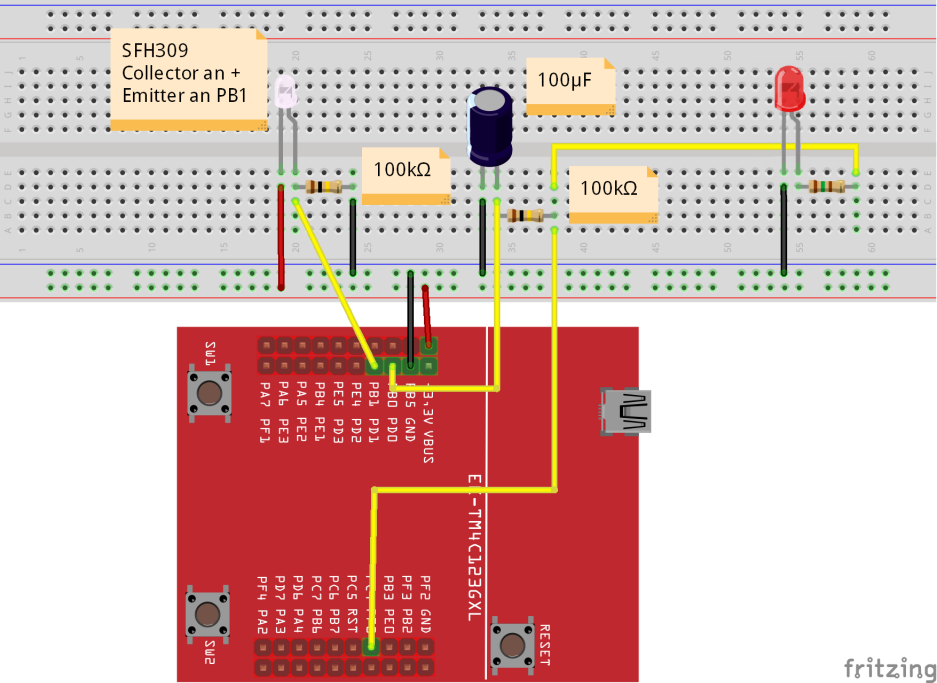
\includegraphics[width=0.7\linewidth]{images/Schaltplan7}
\end{figure}

	
\section{Aufgabe 3}
Programmieren Sie das beschriebene System für das LaunchPad unter strikter Verwendung der FreeRTOS Bibliothek. Damit geht insbesondere ein Verbot der Energie-Funktion \textit{delay()} einher.\\ \\
\textbf{Tipp:} Sie dürfen die GPIO-Funktionen der Energie-Bibliothek, wie z.B. \textit{pinMode()} oder \textit{analogRead()}, verwenden.\\ \\
\textbf{Tipp:} Als Startpunkt liegt ein Eclipse-Projekt im Ilias bereit, das die Onboad-LED des Boards unter Verwendung von FreeRTOS blinken lässt (s. main.cpp).
\definecolor{mygreen}{rgb}{0,0.6,0}
\definecolor{mymauve}{rgb}{0.58,0,0.82}
\lstset{
	breakatwhitespace=false,
	breaklines=true,
	commentstyle=\color{mygreen},
	frame=single,
	keepspaces=true,
	showstringspaces=false,
	keywordstyle=\color{blue},
	language=C,
	rulecolor=\color{black},
	stringstyle=\color{mymauve},
	tabsize=2
}
\lstinputlisting{../FreeRTOSVorlage/src/main.cpp}